In this chapter we explain the process of loading individual levels in our
game. This involves loading the level - encoded as an image in the PNG format -
parsing values from this format, and finally placing tiles in the game world
representing those values.

\section{Loading levels}
Early in the development process, we established that for the type of game we
are making, it is important that we can quickly create levels of varying layout
and sizes, for various reasons, such as:
\begin{itemize}
    \item Our development process, in it being agile. This should afford quick
        turnarounds and iterations, therefore requiring that we can quickly
        produces content for our game, such as levels.
    \item Game balancing, requiring us to produce levels at a sufficient pace in
        order to quickly iterate on game balancing topics, such as strategies
        for a particular map layout.
    \item That we do not have a dedicated level designer on our team, whom we
        could allocate to finely tune and manually design levels.
\end{itemize}

From the above arguments, it is clear that we not only want to produce levels
in a quick manner, but also automate the process of placing
\texttt{gameobjects} in gameworld. While Unity's Editor can for many purposes
be thought of as a \textit{level editor}, we have chosen \textit{not} to use it
for designing levels for the following reasons:
\begin{itemize}
    \item Manually designing levels and placing gameobject in the Editor does
        not afford quick iterations, as required by our development process.
    \item The Editor does not afford easy refactoring of large levels, in that
        objects must be moved or replaced by hand. \textit{Large} is relative,
        but for our purposes it could be upwards +10.000 gameobjects.
    \item Individual levels would have to reside in individual \texttt{Scene}
        files, increasing the complexity of collaboration since scenefiles do
        not merge well in VCSs.
    \item A additional combinatorial complexity is introduced if we decide to
        also support different graphical appearances for objects in a level -
        what one could refer to as \textit{texture packs}. We would have
        to place a gameobject layout for each level for each texture pack.
\end{itemize}

While there are different approaches for circumventing the above
inconveniences, our solution is to encode the layout of each individual level
in an external file which is then loaded and interpreted. Historically, game
developers have often used this approach, usually encoded in some in-house
binary format. While we could have specified our own format, we have chosen to
encode the map in the PNG (Portable Network Graphics) for the following
reasons:
\begin{itemize}
    \item The PNG format is ubiquitous, in that there exists support for it
        almost anywhere, including in Unity3d - both in terms of API and the
        editor itself.
    \item It being ubiquitous means that we do not have to develop additional
        software in order to edit levels - most mainstream image editors
        support the PNG format.
    \item The PNG allows us to encode \textit{enough} information.
        \textit{Enough} being relative, but each colorchannel for each
        individual pixel offers 1 \texttt{byte} of information. With each pixel
        being encoded with RGBA (red, green, blue and alpha) channels, that
        gives us a total of 4 \texttt{bytes} of information.
\end{itemize}

Using the PNG format, it is then only a matter of specifying \textit{what} a
particular color should encode and interpreting that color when loading a
level. As an example, the following could specify how colors could be specified
to encode information about a level:
\begin{itemize}
    \item Black would be ground,
    \item green is grass,
    \item red is building floor, and
    \item yellow being building walls.
\end{itemize}

One obvious shortcoming from the above example is the lack of variation - maybe
one would like to be able to specify different types of walls or floors. This
could however be mitigated by either specifying more colors, by interpreting a
color randomly over a set or by interpreting a color differently depending on
the colors around it. To introduce variety into our levels, we use the latter
approach for some colors, which we will describe later in this chapter.
\\

Having decided on the format and encoded color values, we can design levels
such as seen in figure~\ref{fig:png_map}.

\begin{figure}[H]
    \caption{A PNG image encoding a map}
    \centering
    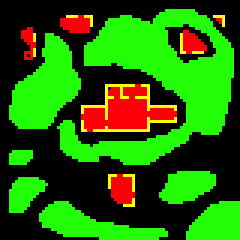
\includegraphics{figures/generating_levels/map.png}
    \label{fig:png_map}
\end{figure}

From figure~\ref{fig:png_map}, we can immediately see that there are some patches
of grass, a building in the middle of the map and some torn-down buildings in
the periphery of the map. Some individual pixels of cyan color can be seen,
which encode where monster should spawn. Likewise, a single white pixel encode
the exit point of the map, which is where players are required to go to when
the missions for this map have been completed. And last, a single blue pixels
encodes where the crafting table should be placed within the level.
\\

(show below how the image is converted into a 2d array)
{\footnotesize
\setlength{\tabcolsep}{2.5pt}
\begin{center}
  \begin{tabular}{|c|c|c|c|c|}
    \hline
    1 & 2 & 3 & 3 & 3 \\ \hline
    4 & 5 & 6 & 3 & 3 \\ \hline
    4 & 5 & 6 & 3 & 3 \\ \hline
    4 & 5 & 6 & 3 & 3 \\ \hline
    7 & 8 & 9 & 3 & 3 \\
    \hline
  \end{tabular}
\end{center}
}
